% Intended LaTeX compiler: pdflatex
\documentclass[11pt]{article}
\usepackage[utf8]{inputenc}
\usepackage[T1]{fontenc}
\usepackage{graphicx}
\usepackage{longtable}
\usepackage{wrapfig}
\usepackage{rotating}
\usepackage[normalem]{ulem}
\usepackage{amsmath}
\usepackage{amssymb}
\usepackage{capt-of}
\usepackage{hyperref}
\author{Fethi Okyar}
\date{2026-05-06}
\title{Chapter 6: Velocity Fields\\\medskip
\large Reading: [Fung/94] Chapter 6}
\hypersetup{
 pdfauthor={Fethi Okyar},
 pdftitle={Chapter 6: Velocity Fields},
 pdfkeywords={},
 pdfsubject={},
 pdfcreator={Emacs 30.2 (Org mode 9.7.11)}, 
 pdflang={English}}
\begin{document}

\maketitle
\setcounter{tocdepth}{1}
\tableofcontents

\section*{(\(\S6.1\)) Velocity Fields}
\label{sec:org4f0ae79}
\subsection*{Fluids}
\label{sec:org046e972}
\begin{itemize}
\item In the study if a fluid, we are generally concerned with the a flow, and it's velocity field. The field of flow is described by the time rate of change in the position vector \(\dot{\boldsymbol{x}}\), called the velocity vector field.
\end{itemize}
\begin{itemize}
\item The velocity components in indicial notation read, \(v_i = v_i(x_1,\,x_2,\,x_3,t)\).
\item The velocity difference between two adjacent points \(P\) and \(P'\) located at \(x_i\) and \(x_i + dx_i\) can be found by invoking the chain rule of differentiation as
$$ dv_i = \frac{\partial v_i}{\partial x_j} dx_j. $$
\item This also corresponds to the operation
$$ d\boldsymbol{v} = d\boldsymbol{x} \cdot \nabla\boldsymbol{v} $$
where \(\nabla\boldsymbol{v}\) is known as the \emph{velocity gradient} tensor.
\end{itemize}
\subsubsection*{Cartan Decomposition of the Velocity Gradient}
\label{sec:orgb4b2f5b}
The \emph{Cartan} decomposition of the velocity gradient vector yields
  $$ \frac{\partial v_i}{\partial x_j} = \frac{1}{2} \left( \frac{\partial v_i}{\partial x_j} + \frac{\partial v_j}{\partial x_i} \right) +  \frac{1}{2} \left( \frac{\partial v_i}{\partial x_j} - \frac{\partial v_j}{\partial x_i} \right) $$
  where the left term on the right hand side is a symmetric tensor and the one on the right is a skew-symmetric tensor.
\subsection*{Definitions}
\label{sec:org47a0db1}
\begin{itemize}
\item The symmetric part of the velocity gradient is the rate of deformation tensor, (or the deformation rate tensor)
$$ V_{ij} \equiv  \frac{1}{2} \left( \frac{\partial v_i}{\partial x_j} + \frac{\partial v_j}{\partial x_i} \right), $$
\end{itemize}
\begin{itemize}
\item while the skew-symmetric part is called the spin tensor
$$ \Omega_{ij} \equiv \frac{1}{2} \left( \frac{\partial v_i}{\partial x_j} - \frac{\partial v_j}{\partial x_i} \right). $$
\item Then
$$ \frac{\partial v_i}{\partial x_j} = V_{ij} + \Omega_{ij} $$
\item Evidently, \(V_{ij}\) is symmetric and \(\Omega_{ij}\) is skew-symmetric
$$ V_{ij} = V_{ji}, \hspace{2em} \Omega_{ij} = -\Omega_{ji}. $$
\end{itemize}
\subsection*{Vorticity}
\label{sec:org71de79e}
\begin{itemize}
\item The tensor \(\Omega_{ij}\) has only three independent (non-zero) elements
$$ [\Omega_{ij}] = \begin{bmatrix} 0 & \Omega_{12} & \Omega_{13} \\ -\Omega_{12} & 0 & \Omega_{23} \\ -\Omega_{13} & -\Omega_{23} & 0 \end{bmatrix} $$
\end{itemize}
\begin{itemize}
\item There exists a vector \(\boldsymbol{\omega}\) dual to \(\boldsymbol{\Omega}\); that is
$$ \omega_k \equiv \varepsilon_{kij} \Omega_{ij}; \hspace{2em} \mathrm{i.e.} \hspace{2em} \boldsymbol{\omega} = \nabla \times \boldsymbol{v} = \mathrm{curl}\,\boldsymbol{v} $$
where \(\varepsilon_{kij}\) is the permutation tensor, and the vector \(\boldsymbol{\omega}\) is called the \emph{vorticity} vector.
\end{itemize}
\subsubsection*{Query AI:}
\label{sec:orgedf0d65}
\begin{verbatim}
Provide a clear definition of vorticity in a flow field.
If possible, provide illustrations or suggest references or sources
that point graphical illustrations depicting vorticity.
\end{verbatim}
\subsection*{Problems}
\label{sec:org7602f6c}
\subsubsection*{6.1}
\label{sec:org83b7a6f}
\begin{center}
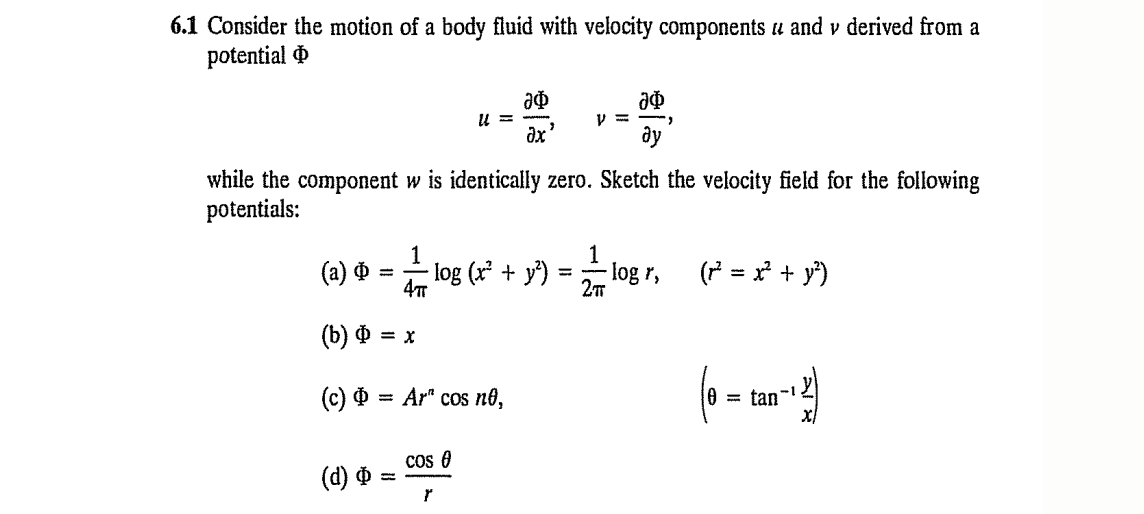
\includegraphics[width=.9\linewidth]{./images/FU94_6.1problem1.png}
\end{center}
\end{document}
